\documentclass[times, 9pt,twocolumn]{article} 
\usepackage[utf8]{inputenc}
\usepackage[ngerman]{babel}
\usepackage{comment}
\usepackage{times}
\usepackage{geometry}
\usepackage{fancyhdr}
\usepackage{amsmath ,amsthm ,amssymb}
\usepackage{graphicx}
\usepackage{hyperref}
\usepackage{comment}
\usepackage{apacite}
\usepackage{bm}
\usepackage[mode=buildnew]{standalone}
\usepackage{tikz}
\usepackage{booktabs}
\usepackage{siunitx}
\bibliographystyle{apacite}

% tikz commands because otherwise the standalone compiling doesnt work
\usetikzlibrary{positioning}
\usetikzlibrary{calc}
\usetikzlibrary{arrows.meta}
\tikzset{
  arr/.style={{Circle[length=3pt]}->,shorten <=-1.5pt}
}

% Eigene Makros
\DeclareMathOperator{\diag}{\mathrm{diag}}
\newcommand{\partiell}[3][]{\frac{\partial^{#1}#2}{\partial{#3}^{#1}}}
\newcommand{\diff}[3][]{\frac{\mathrm{d}^{#1}#2}{\mathrm{d}{#3}^{#1}}}
\newcommand{\dr}{\mathrm{d}}
\newcommand{\vect}[1]{\boldsymbol #1}
\newcommand{\Reals}{\mathds R}
\newcommand{\Compl}{\mathds C}
\DeclareMathOperator{\Real}{\mathfrak R}
\DeclareMathOperator{\Imag}{\mathfrak I}
\newcommand{\norm}[1]{\left\|#1\right\|}
\newcommand{\abs}[1]{\left|#1\right|}
\newcommand{\skalprod}[2]{\langle#1,#2\rangle}
\DeclareMathOperator{\grad}{\mathrm{grad}}
\DeclareMathOperator{\sgn}{\mathrm{sgn}}
\renewcommand{\div}{\mathrm{div}}
\DeclareMathOperator{\rang}{rang}

\pagestyle{empty}
\begin{document}
	\title{Oberseminar Regelungstechnik \\ Regler- und Kalmanfilterentwurf f\"ur einen 					Helikopterversuchstand}
	\author{Tilo Stock, Clemens Bilsing, Robert Heedt}
	\date {29.03.2019}

	\maketitle
	\thispagestyle{empty}
	% Das Inhaltsverzeichnis sieht in diesem Stil nicht gut aus. Soll es überhaupt dazu? 
	% Immerhin ist ein Tagungsbericht kein Buch. 
	% \tableofcontents
	% \newpage
	
	\renewcommand\abstractname{Zusammenfassung}
	\begin{abstract}
		%Dies ist ein ziemlich abstraktiges Abstrakt.
		In dieser Projektarbeit wurde das nachfolgend abgebildete Helikopterexperiment mathematisch modelliert und verschiedene Reglerstrategien zur Arbeitspunkt- und Folgeregelung untersucht.
		Weiterhin wurde zur Zustandsrekonstruktion ein Kalmanfilter entworfen. Alle Ergebnisse wurden in einer interaktiven Simulationsumgebung implementiert und visualisiert.

		\begin{figure}[ht]
			\centering
			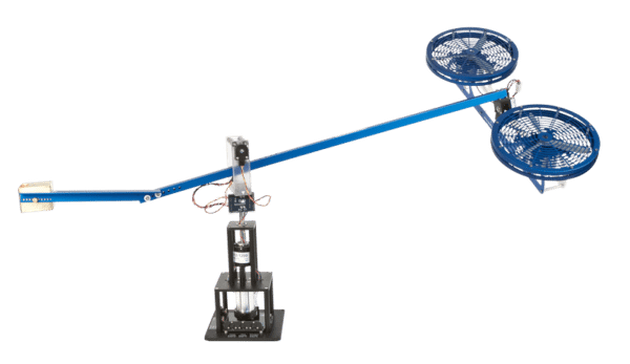
\includegraphics[width=0.4\textwidth]{images/Versuchstand}
			\caption{Versuchsstand des Helikopterexperiments}
			\label{Versuchstand}
		\end{figure}
	\end{abstract}
	
	\section{Modellbildung}
	\subsection{Einführung}

	Als erster Schritt der Modellbildung wurde der komplexe Versuchstand stark vereinfacht und auf drei Punktmassen reduziert. Davon repräsentieren zwei die Motoren, welche die Propeller antreiben um Auftrieb zu erzeugen. Die dritte Punktmasse repräsentiert das Gegengewicht der Motoren. Weiterhin verfügt das System über drei Gelenke um den Helikopterkopf im Raum bewegen zu können.

	\begin{figure}[ht]
		\centering
		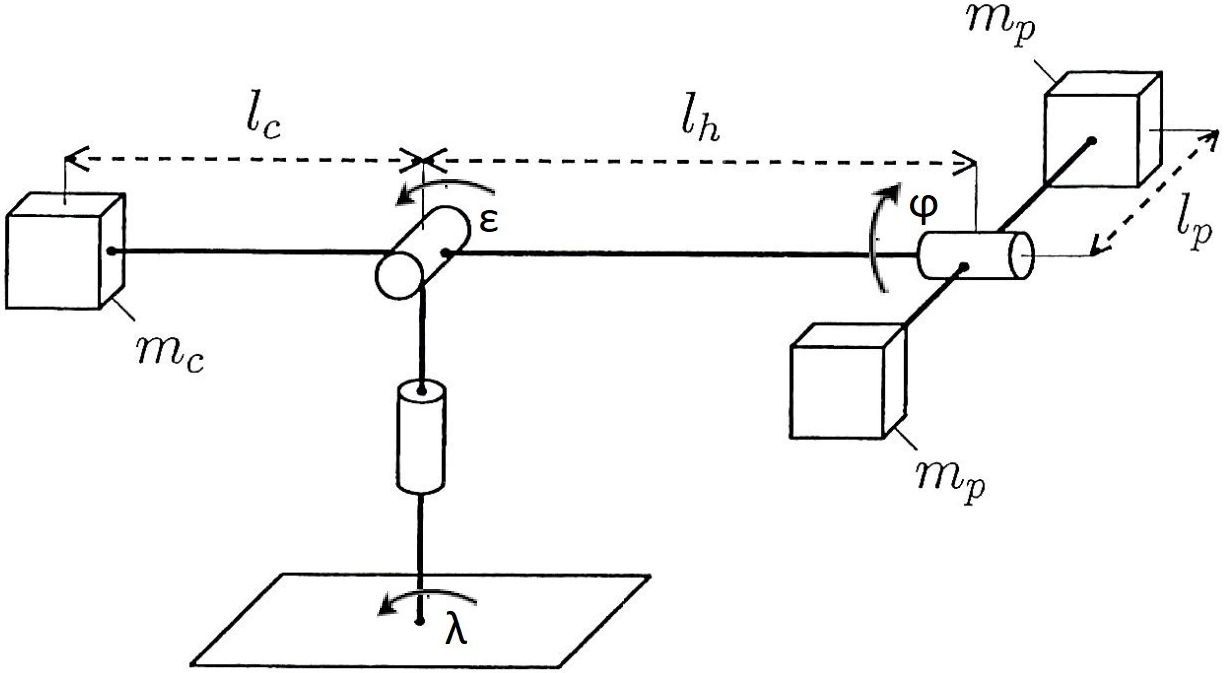
\includegraphics[width=0.5\textwidth]{images/setup}
		\caption{Vereinfachter Versuchsstand}
		\label{setup}
	\end{figure}
	Das Koordinatensystem des Modells wurde durch seine generalisierten Koordinaten folgendermaßen festgelegt: $\bm q = \begin{bmatrix}
	\varphi & \varepsilon & \lambda
	\end{bmatrix}^T $

	\subsection{Langrange-Formalismus}

	Um die Bewegungsgleichungen des Modells zu bestimmen bietet sich der Lagrange-Formalismus zweiter Art besonders an. Für Systeme mit generalisiertem Potential lautet die Lagrange-Gleichung $L = T -V$ wobei $T$ jeweils die kinetische und $V$ die potentielle Energie des System bezeichnen.
	Mit der Betrachtung von nicht-konservativen Kräften $Q_i$ ergibt sich die Lagrange-Funktion
	\begin{equation}\label{eq:lagrange}
	\diff{}{t} \partiell{L}{\dot{q_i}} - \partiell{L}{q_i}=Q_i\, .
	\end{equation}
	Nach Einsetzen der potentiellen und kinetischen Energien sowie der nicht-konservativen Kräfte des Systems ergeben sich folgende Bewegungsgleichungen:
	\begin{equation}
	\begin{split}
	&J_\varphi \ddot{\varphi} - J_\varphi \cos (\varphi) \sin (\varphi) (\dot{\varepsilon}^2- \cos^2 (\varepsilon) \dot{\lambda}^2)\\  &+ \mu_\varphi \dot{\varphi} = V_d L_1
	\end{split}
	\end{equation}
	\begin{equation}
	\begin{split}
	&J_\varepsilon(\varphi)\ddot{\varepsilon} + \mu_\varepsilon \dot{\varepsilon} + J_\varepsilon(\varphi) \cos (\varepsilon) \sin (\varepsilon) \dot{\lambda}^2\\
	&= L_2 \cos \varepsilon + V_s L_3 \cos \varphi
	\end{split}
	\end{equation}
	\begin{equation}
	J_\lambda(\varepsilon,\varphi) \ddot{\lambda} + \mu_\lambda \dot{\lambda} = V_s L_4 \cos \varepsilon \sin \varphi
	\end{equation}
	Mit $J_i$ .. Trägheitsmoment um Achse $i$; $V_s$ .. Summe der Rotorspannung $V_f + V_b$; $V_d$ .. Differenz der Rotorspannungen $V_f - V_b$; $L_i$ .. Längenkonstante; $\mu_i$ .. Gleitreibungskoeffizient um Gelenk $i$. Dieses einfache Modell beinhaltet bereits Zentripetalkräfte sowie Gleitreibung der Gelenke.

%	\subsection{Langrange-Formalismus (long)}
%
%	Um die Bewegungsgleichungen des Modells zu bestimmen bietet sich der Lagrange-Formalismus zweiter Art besonders an. Für Systeme mit generalisiertem Potential lautet die Lagrange Gleichung $L = T -V$ wobei $T$ jeweils die kinetische und $V$ die potentielle Energie des System bezeichnen.
%	Mit der Betrachtung von nicht-konservativen Kräften $Q_i$ ergibt sich die Lagrange-Funktion
%	\begin{equation}\label{eq:lagrange}
%	\diff{}{t} \partiell{L}{\dot{q_i}} - \partiell{L}{q_i}=Q_i
%	\end{equation}
%	Zur Bestimmung der kinetischen Energie $T$ wurde die Rotation jeder einzelnen Masse um jede Koordinatenachse betrachtet und aufsummiert. Zusammengefasst ergibt sich
%	\begin{equation}
%	\begin{split}
%	T&= m_p l_p^2\dot{\varphi}^2 \\
%	&+ \frac{1}{2}m_cl_c^2\dot{\varepsilon}^2
%	+ m_p(l_h^2+(l_p\sin \varphi)^2)\dot{\varepsilon}^2\\
%	&+ \frac{1}{2} m_c (l_c \cos \varepsilon)^2\dot{\lambda}^2\\
%	&+ m_p((l_h \cos \varepsilon)^2 + (l_p \sin \varphi \sin \varepsilon)^2\\
%	&+(l_p \cos \varphi)^2)\dot{\lambda}^2
%	\end{split}
%	\end{equation}
%	Die potentielle Energie $V$ lautet
%	\begin{equation}
%	V = -m_c l_c g \sin \varepsilon + 2 m_p l_h g \sin \varepsilon
%	\end{equation}
%	Die durch die Rotation der Rotoren sowie durch Gleitreibung entstehen nicht-konservative Kräfte, welche wie folgt vereinfacht dargestellt werden können:
%	\begin{align}
%	Q_\varphi &= (F_f - F_b)l_p - \mu_\varphi \dot{\varphi} \\
%	Q_\varepsilon &= (F_f + F_b)l_h  \cos \varphi - \mu_\varepsilon \dot{\varepsilon}\\
%	Q_\lambda &= (F_f + F_b)l_h \cos \varepsilon \sin \varphi - \mu_\lambda \dot{\lambda}
%	\end{align}
%	Eingesetzt in \eqref{eq:lagrange} wurde durch zeitliche und räumliche Ableitung nach jeder generalisierten Koordinate folgende Bewegungsgleichungen bestimmt:
%	\begin{equation}
%	\begin{split}
%	&J_\varphi \ddot{\varphi} - J_\varphi \cos (\varphi) \sin (\varphi) (\dot{\varepsilon}^2- \cos^2 (\varepsilon) \dot{\lambda}^2)\\  &+ \mu_\varphi \dot{\varphi} = V_d L_1
%	\end{split}
%	\end{equation}
%	\begin{equation}
%	\begin{split}
%	&J_\varepsilon(\varphi)\ddot{\varepsilon} + \mu_\varepsilon \dot{\varepsilon} + J_\varepsilon(\varphi) \cos (\varepsilon) \sin (\varepsilon) \dot{\lambda}^2\\
%	&= L_2 \cos \varepsilon + V_s L_3 \cos \varphi
%	\end{split}
%	\end{equation}
%	\begin{equation}
%	J_\lambda(\varepsilon,\varphi) \ddot{\lambda} + \mu_\lambda \dot{\lambda} = V_s L_4 \cos \varepsilon \sin \varphi
%	\end{equation}
%	Mit $J_i$ .. Trägheitsmoment um Achse $i$; $V_s$ .. Summe der Rotorspannung $V_f + V_b$; $V_d$ .. Differenz der Rotorspannungen $V_f - V_b$; $L_i$ .. Längenkonstante; $\mu_i$ .. Gleitreibungskoeffizient um Gelenk $i$. Dieses einfache Modell beinhaltet bereits Zentripetalkräfte sowie Gleitreibung der Gelenke.

	\subsection{Motordynamik}

	Weiterhin wurde das Modell um die Rotordrehzahlen $\omega$ der Motoren erweitert. Diese ergeben sich aus der jeweiligen Motorspannung $V$ mittels Tiefpass 1. Ordnung:
	\begin{subequations}
	\begin{align}
	T_f \dot{\omega_f} + \omega_f &= K_f V_f\\
	T_b \dot{\omega_b} + \omega_b &= K_b V_b\, .
	\end{align}
\end{subequations}

	\begin{figure}[ht]
	\centering
	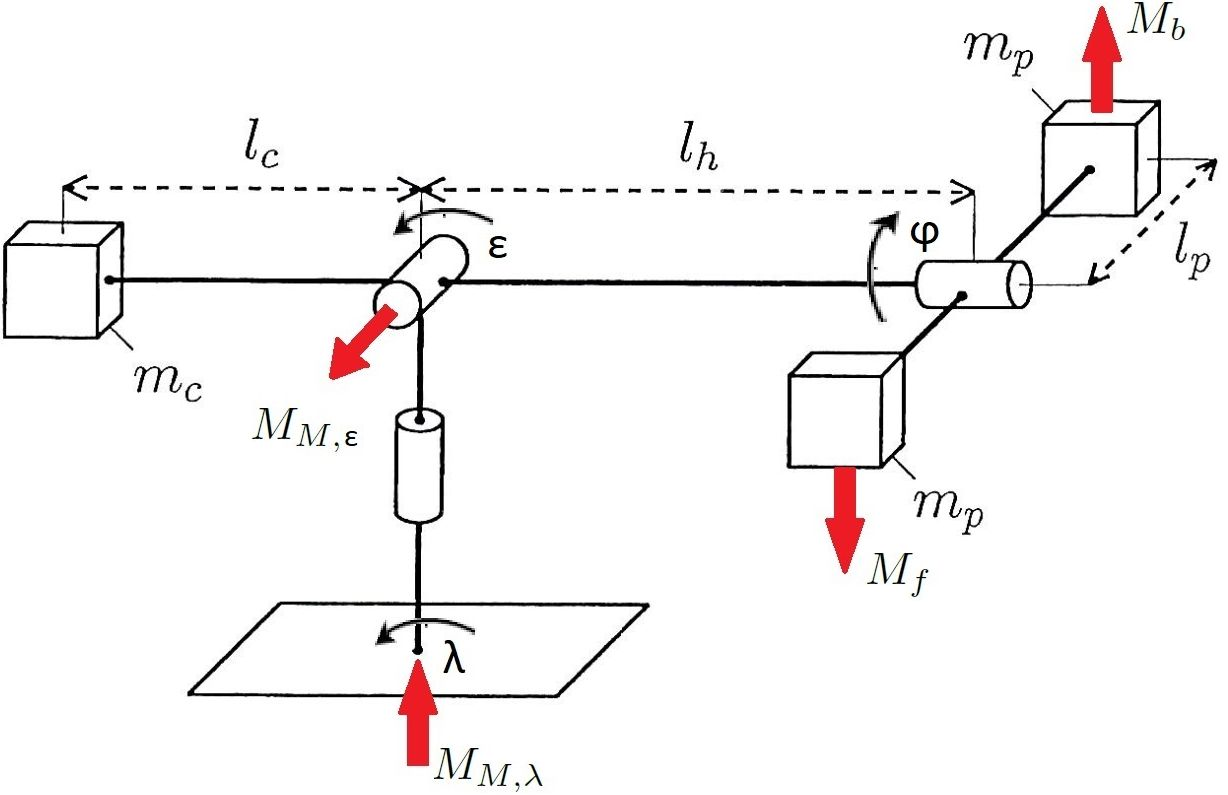
\includegraphics[width=0.5\textwidth]{images/setup_mom}
	\caption{Reaktionsmomente der Gelenke}
	\label{setup_mom}
	\end{figure}
	Weiterhin entsteht ein Reaktionsmoment der Motoren auf die Gelenke. Um diesen parasitären Effekt zu minimieren wurde angenommen, dass die Rotoren standardmäßig entgegengesetzt rotieren. Die entstandenen Reaktionsmomente können beschrieben werden durch:
	\begin{subequations}		
	\begin{align}
	M_{M,\varepsilon} &=\sin (\varphi) K_M (\omega_f-\omega_b) \\
	M_{M,\lambda} &=\cos (\varepsilon) \cos (\varphi) K_M (\omega_b-\omega_f)\, .
	\end{align}
\end{subequations}


	\subsection{Kreiseleffekte}

	Zusätzlich wirken Kreiselmomente auf die Rotoren, wenn sich die Rotationsachse der Rotoren verändert. Diese Kreiselmomente können allgemein beschreiben werden durch:
	\begin{equation}
	\vec{M} = \vec{\Omega} \times \vec{L}\, .
	\end{equation}	
	Angewandt auf Rotation um $\varphi$:
	\begin{subequations}
		\begin{align}
		&M_{K\varepsilon,\varphi} = J_M \cos (\varphi) \dot{\varphi}(\omega_f-\omega_b)\\
		&M_{K\lambda,\varphi} = J_M \sin (\varphi) \cos (\varepsilon) \dot{\varphi}(\omega_f-\omega_b)\, .
		\end{align}
	\end{subequations}
	Angewandt auf Rotation um $\varepsilon$:
	\begin{equation}
	M_{K\varphi,\varepsilon} = J_M \cos (\varphi) \dot{\varepsilon}(\omega_b-\omega_f)\, .
	\end{equation}
	Angewandt auf Rotation um $\lambda$:
	\begin{subequations}
		\begin{align}
		&M_{K\varphi,\lambda} = J_M \sin (\varphi) \cos (\varepsilon) \dot{\lambda}(\omega_f-\omega_b)\\
		&M_{K\varepsilon,\lambda} = J_M \cos (\varphi) \sin (\varepsilon) \dot{\lambda}(\omega_b-\omega_f)\, .
		\end{align}
	\end{subequations}

	\subsection{Modellvalidierung}

	Es wurden einige zusätzliche Experimente implementiert um die Bewegungsgleichungen des Modells zu validieren. Dazu wurde vor allem auf die Validierung des einfachsten Modells eingegangen, das durch den Langrange-Formalismus bestimmt wurde.
	Dazu wurde in einem Experiment die Winkelgeschwindigkeit des Helikopterkopfes extern eingestellt ($\dot{\lambda} = \mathrm{const}$) und die Propeller ausgestellt ($V_f = V_b = 0$).
	Dazu wurde analytisch die Ruhelage der anderen Gelenkwinkel in Abhängigkeit von $\dot{\lambda}$ berechnet und mit der Simulation verglichen.
	Interessant ist dabei, dass sich der Helikopterkopf durch die wirkenden Zentripetalkräfte nach einiger Zeit immer horizontal ausrichtet.
	
	\section{Regelung}
	\subsection{Arbeitspunktregelung}
	%Aus regelungstechnischer Sicht sind besonders zwei Aufgaben interessant: zum Einen die Stabilisierung des Systems an einem definierten Arbeitspunkt, beschrieben in diesem Abschnitt, und zum Anderen die Folgeregelung, bei der die Systemzustände einem Sollverlauf folgen sollen.
	\subsubsection{Heuristisch durch PID-Regler}
	%Einfache PID-Regler sind für viele praktische Probleme in der Lage, auch ohne umfangreiche mathematische Modellierung und Berechnung, durch geschickte Handeinstellung Ruhelagen zu stabilisieren.
	%Deshalb liegt auch hier nahe, einen solchen Ansatz auszuprobieren.
    %
	Eine Ruhelage in diesem System kann durch zwei frei wählbare Winkel \(\varepsilon^* \in (-\frac{\pi}{2}, \frac{\pi}{2})\) und \(\lambda^* \in (-\pi, \pi)\) beschrieben werden, außerdem gilt \(\varphi^*=0\).
	Zur Einstellung der Ruhelage stehen als Stellgrößen die Motorspannungen \(V_f\) für den vorderen, und \(V_b\) für den hinteren Motor zur Verfügung.

	Ein PID-Regler der Form
	\[
		y(t) = k_P x(t) + k_I \int_0^t x(t') \, \mathrm{d}t' +  k_D \dot{x}(t)
	\]
	besitzt nur jeweils einen skalaren Eingang und Ausgang, für dieses System müssen also mehrere miteinander verschaltet werden.
	
	Der vollständige Regelkreis ist in Abbildung~\ref{fig:pid_diagram} dargestellt.
	PID~1 und~2 setzen Drehzahlvorgaben in Motorspannungen um, PID~3 realisiert einen internen Sollwert für \(\varphi\), und 4 und 5 die äußeren Vorgaben für \(\varepsilon\) und \(\lambda\).
	Die Transformation
	\begin{equation}
		\omega_f = \frac{\omega_s+\omega_d}{2}, \quad
		\omega_b = \frac{\omega_s-\omega_d}{2}
	\end{equation}
	bewirkt eine teilweise Entkopplung zwischen den Einflüssen der Stellgrößen auf die Zustände, sodass allein über \(\omega_d\) der Winkel \(\varphi\) eingestellt werden kann.
	Die Vorsteuerung ist nicht zwangsweise nötig, führt aber zu einer etwas besseren Dynamik, da die Ruhedrehzahl \(\omega_s^0 \neq 0\) für \(\varepsilon^* \neq 0\) nicht vom I-Anteil des PID~4 übernommen werden muss.
	
	In den Simulationen waren die Regler so in der Lage, Anfangsfehler von ca. \ang{30} in den Winkeln, sowie kleine Störmomente auszugleichen.
	%Mit der beispielhaften Parametrierung in \ref{tab:pid_parameters} sind die Regler in der Lage, Anfangsfehler von ca. \ang{30} in den Winkeln, sowie kleine Störmomente auszugleichen.
	% Noch iwie Messwerte oder Diagramme?
	\begin{figure*}
		\centering
		\includestandalone[scale=0.9]{pid_diagram}
		\caption{Struktur der Arbeitspunktregelung mit PID-Reglern}
		\label{fig:pid_diagram}
	\end{figure*}
	% \begin{table}
	% 	\centering
	% 	\begin{tabular}{l l l l}
	% 		\toprule
	% 		PID & $k_P$ & $k_I$ & $k_D$\\
	% 		\midrule
	% 		1 & 5 & 0 & 0\\
	% 		2 & 5 & 0 & 0\\
	% 		3 & 20 & 0 & 6\\
	% 		4 & 10 & 6 & 5\\
	% 		5 & 2 & 0,6 & 2\\
	% 		\bottomrule
	% 	\end{tabular}
	% 	\label{tab:pid_parameters}
	% 	\caption{Beispielhafte PID-Parametrierung}
	% \end{table}
	\subsubsection{Konstante Zustandsrückführung}
	Um auf die Methoden der linearen Regelungstechnik zurückgreifen zu können, wird das nichtlineare System
	\begin{equation}
		\dot{\vect x} = \vect f(\vect x, \vect u)
	\end{equation}
	zuerst analytisch linearisiert und am Arbeitspunkt \(\vect{x}^*\), \(\vect{u}^*\) ausgewertet, sodass man die Systemmatrizen
	\begin{equation}
		\vect{A} = \left. \partiell{\vect f}{\vect x}\right\vert_\mathrm{AP}, \quad
		\vect B = \left. \partiell{\vect f}{\vect u}\right\vert_\mathrm{AP}
	\end{equation}
	für das lineare Entwurfssystem in Zustandsraumdarstellung
	\begin{equation}
		\dot{\tilde{\vect{x}}} = \vect A \tilde{\vect{x}} + \vect B \tilde{\vect{u}}
	\end{equation}
	mit den Differenzgrößen
	\(
		\tilde{\vect{a}} = \vect{a} - \vect{a}^*
	\)
	erhält.

	Um eine stabilisierende Rückführung \(\tilde{\vect{u}} = - \vect{K} \tilde{\vect{x}}\) zu entwerfen, wurden zwei Varianten implementiert.
	Einerseits können Eigenwerte für die Systemmatrix mit Rückführung \(\vect A - \vect K \vect B\) vorgegeben werden.
	Andererseits kann die Methode des LQR-Entwurfes genutzt werden, bei der ein Kostenfunktional
	\[
		J = \int^{\infty}_0 x(t)^T Q\, x(t) + u(t)^T R\, u(t)\ \mathrm dt
	\]
	mit diagonalen Wichtungsmatrizen \(\vect Q\) und \(\vect R\) minimiert wird.

	Interessanterweise war dieser Regler auch bei großen Abweichungen, wie zum Beispiel \ang{120} in \(\lambda\), mithilfe der Winkelbeschränkung von \(\varphi\) noch in der Lage, den Arbeitspunkt zu erreichen.
	\subsection{Folgeregelung}
	\subsubsection{Flachheitsbasierter Ansatz}
	Ein vereinfachtes Systemmodell ohne Motordynamik und Kreiseleffekte
% 	\begin{subequations}
% 		\begin{align}
% J_\varphi \ddot{\varphi} &= L_1 \omega_d\\
% J_\varepsilon \ddot{\varepsilon} &= L_2 \cos (\varepsilon) + L_3 \omega_s \cos (\varphi)\\
% J_\lambda \ddot \lambda &= L_4 \omega_s \sin (\varphi) \cos (\varepsilon)
% 		\end{align}
% 	\end{subequations}
	\begin{subequations}
		\begin{align}
			J_\varphi \ddot{\varphi} +\mu_\varphi \dot \varphi - M_{z,\varphi} &= L_1 \omega_d
			\label{eq:flat1}\\
J_\varepsilon \ddot{\varepsilon} + \mu_\varepsilon \dot\varepsilon + M_{z, \varepsilon} &= L_3 \omega_s \cos (\varphi)
\label{eq:flat2}\\
J_\lambda \ddot \lambda + \mu_\lambda \dot\lambda &= L_4 \omega_s \sin (\varphi) \cos (\varepsilon)
\label{eq:flat3}
		\end{align}
	\end{subequations}
	mit den Zentripetalmomenten
	\begin{subequations}
		\begin{align}
			M_{z,\varphi} &= J_\varphi \cos(\varphi) \sin(\varphi) (\dot \varepsilon^2-\cos^2(\varepsilon) \dot \lambda^2)\\
			M_{z, \varepsilon} &= J_\varepsilon \cos(\varepsilon) \sin(\varepsilon) \dot\lambda^2 - L_2 \cos (\varepsilon)
		\end{align}
	\end{subequations}
	besitzt den flachen Ausgang
	\(
		\vect y = (\varepsilon, \lambda)
	\)
	und lässt sich in die Regelungsform
	% \begin{subequations}
	% 	\begin{align}
	% 		\omega_s &= \Phi_1(\varepsilon, \ddot \varepsilon, \ddot \lambda)\\
	% 		\omega_d &= \Phi_2(\varepsilon, \dot \varepsilon, \ddot \varepsilon, \varepsilon^{(3)}, \varepsilon^{(4)}, \ddot \lambda, \lambda^{(3)}, \lambda^{(4)})\, .
	% 	\end{align}
	% \end{subequations}
	%Es lässt sich zeigen, dass eine Regelungsform
	\begin{subequations}
		\begin{align}
			\varepsilon^{(4)} &= \Psi_1(\omega_s, \dot{\omega}_s, \ddot{\omega}_s, \omega_d)\\
			\ddot \lambda &= \Psi_2(\omega_s, \dot{\omega}_s, \ddot{\omega}_s, \omega_d)
		\end{align}
	\end{subequations}
	%existiert.
	transformieren.
	Um jetzt aber eine stabilisierende Rückführung
	\[
		\varepsilon^{(4)} = \varepsilon_d^{(4)} - \sum_{i=0}^3 k_i (\varepsilon^{(i)} - \varepsilon_d^{(i)})
	\]
	zu berechnen, die dazu führt, dass \(\varepsilon(t)\) dem Verlauf \(\varepsilon_d(t)\) folgt, werden die dritten und vierten zeitlichen Ableitungen von \(\varepsilon\) benötigt, die in unserer Simulation nicht zur Verfügung stehen.
	Um das Problem zu lösen sollten Verfahren zur Ableitungsschätzung, wie Automatisches Differenzieren, genauer untersucht werden.
	\subsubsection{Linearisierende Rückführung}
	Bei Betrachtung der vereinfachten Systemgleichungen fällt auf, dass $\varphi$ alleine über~\ref{eq:flat1} mit Steuerung von $\omega_d$ bestimmt wird.
	Gehen wir also davon aus, dass ein unterlagerter Regler $\varphi$ ausreichend schnell wie gewünscht einstellt, können wir uns nachfolgend auf das Teilsystem \ref{eq:flat2}-\ref{eq:flat3} beschränken, in dem $\omega_s$ und $\varphi$ als Stellgrößen vorliegen.
	Durch die erste Eingangstransformation
	\begin{equation}
		w_1 = \omega_s \cos(\varphi), \quad
		w_2 = \omega_s \sin(\varphi)
	\end{equation}
	treten die neuen Eingänge affin in den Systemgleichungen auf.
	Indem $(v_1, v_2)$ als zweites Paar virtueller Eingänge definiert wird, kann mit der zweiten Eingangstransformation
	\begin{subequations}
		\begin{align}
			w_1 &= \frac{J_\varepsilon v_1 + \mu_\varepsilon \dot \varepsilon + J_\varepsilon \cos(\varepsilon) \sin(\varepsilon)\dot{\lambda}^2-L_2 \cos(\varepsilon)}{L_3} \\
			w_2 &= \frac{J_\lambda v_2 + \mu_\lambda \dot \lambda}{L_4 \cos{\varepsilon}}
		\end{align}
		\label{eq:linearizing_transformation}
	\end{subequations}
	das Teilsystem \ref{eq:flat2}~-~\ref{eq:flat3} eingangs-zustands-linearisiert werden.

	Nun ist es möglich, für das lineare System
	\begin{subequations}
		\begin{align}
			\ddot{\varepsilon} &= v_1\\
			\ddot{\lambda} &= v_2
		\end{align}
	\end{subequations}
	eine Rückführung zu entwerfen, die Sollverläufen $\varepsilon_d$, $\lambda_d$ folgt.
	Danach kann mit \ref{eq:linearizing_transformation} zurückgerechnet werden und mit
	\begin{subequations}
		\begin{align}
\omega_s &= \sqrt{w_1^2 + w_2^2}\ \sgn (w_1)\\
\varphi_d &= \arctan \left(\frac{w_1}{w_2}\right) 
		\end{align}
	\end{subequations}
	erhält man \(\omega_s\) und einen Sollwert für \(\varphi\).
	Zuletzt wird mit einem PD-Regler über Steuerung von \(\omega_d\) in~\ref{eq:flat1} der Verlauf \(\varphi_d\) realisiert.

	In der Simulation konnten Überführungen zwischen beliebigen Arbeitspunkten mit polynomialen Trajektorien durchgeführt werden.
	Bei zu hohen Geschwindigkeiten führten aber die nicht im Regler berücksichtigten Reaktionsmomente zu einem destabilisierenden Feedback-Effekt.
	Zukünftig sollte also am echten Versuchsstand getestet werden, in welcher Größenordnung dieser Effekt tatsächlich existiert oder alternativ nach einem robusten Regleransatz gesucht werden.

	
	\section{Zustandsrekonstruktion}
	\subsection{Einf\"uhrung}
	Einige Regler verwenden eine Zustandsr\"uckf\"uhrung zur Stabilisierung des Systems. Die Zust\"ande des Systems sind die drei Winkelgr\"oßen, deren Ableitungen und die Rotationsfrequenzen der beiden Motoren. Insofern diese 8 Gr\"oßen nicht direkt gemessen werden, ist eine Echtzeit-Rekonstruktion der Zustände notwendig. 
	Selbst wenn tatsächlich alle Zustände als Messgrößen zur Verfügung stehen sollten, kann es bei starkem Messrauschen sinnvoll sein, die Messsignale mit einem Zustandsschätzer zu glätten.

	Im folgenden Abschnitt wird in diesem Zusammenhang der Entwurf und die Implementierung eines diskreten, Erweiterten Kalman-Filters (\textit{EKF})  thematisiert. 
	\subsection{Detektierbarkeit der Modellgleichungen}
	Damit der Zustandsschätzer überhaupt konvergieren kann, muss das System lokal detektierbar sein. Dies kann durch Linearisierung des Systems und durch Anwendung des Kalmanschen Beobachtbarkeitskriterium nachgewiesen werden. Dabei werden die nichtlinearen Systemgleichungen
	$$ \bm{\dot x} = \bm{f}(\bm{x},\bm{u}),\quad \bm y = \bm{g}(\bm{x}, \bm u) $$
	in einem Arbeitspunkt linearisiert, sodass das System lokal als lineare Näherung durch die Systemgleichungen
	$$ \bm{\dot x} = \bm{A} \bm{x} + \bm{B} \bm{u},\quad \bm y = \bm C \bm x + \bm D \bm u $$
	mit den Matrizen $ \bm A = \frac{\partial{ \bm f}}{\partial{\bm x}}$, $\bm B = \frac{\partial{ \bm f}}{\partial{\bm u}}$, $\bm C = \frac{\partial{ \bm g}}{\partial{\bm x}}$ und $\bm D = \frac{\partial{ \bm g}}{\partial{\bm u}}$ dargestellt werden kann.
	
	Im Folgenden soll die lokale Detektierbarkeit für drei unterschiedliche Fälle nachgewiesen werden:
	\begin{enumerate}
		\item für das einfachste Modell mit den drei gemessenen Gelenkwinkeln als Systemausgang
		\item für das komplexeste Modell mit den drei gemessenen Gelenkwinkeln und den zwei Motorfrequenzen als Systemausgang
		\item für das komplexeste Modell mit den drei gemessenen Gelenkwinkeln, aber ohne den beiden Motorfrequenzen als Systemausgang
	\end{enumerate}
	
	Zur Linearisierung des Systems sowie zur Berechnung der Kalmanschen Beobachtbarkeitsmatrix wurde das CAS von Matlab verwendet, da die Rangberechnung symbolischer Matrizen unter \textit{SymPy} unzumutbar lange dauerte. Dies geschah ohne Wissen von dem Paket \textit{symbtools} von Dr. Knoll, welches einen anderen Algorithmus zur Rangbestimmung symbolischer Matrizen enthält. 
	\subsubsection{Einfachstes Modell}
	Das einfachste Modell folgt aus den Gleichungen 2-4, wenn die Zentripetal- und Reibungskräfte vereinfacht als sehr klein bzw.\ 0 angenommen werden.
	\begin{align*}
	\bm f(\bm x) &= \begin{bmatrix}
	\dot \varphi \\
	\dot \varepsilon \\
	\dot \lambda  \\
	\dfrac{1}{J_p} \cdot L_1 V_d \\
	\dfrac{1}{J_e} \cdot (L_2 \cdot \mathrm{cos(\varepsilon)} + L_3 V_s \mathrm{cos(\varphi)}) \\
	\dfrac{1}{J_{\lambda}} \cdot L_4 V_s \mathrm{cos(\varepsilon)} \mathrm{sin(\varphi)} \\
	\end{bmatrix}\\
	\bm x &= \begin{bmatrix}
	\varphi & \varepsilon & \lambda & \dot \varphi & \dot \varepsilon & \dot \lambda 
	\end{bmatrix}^T \\
	\bm y &= \begin{bmatrix}
	\varphi & \varepsilon & \lambda 
	\end{bmatrix}^T
\end{align*}
	Die Kalmansche Beobachtbarkeitsmatrix
	$$\bm O = \begin{bmatrix}
	\bm C \\
	\ldots \\
	\bm C \bm A^{n-1}
	\end{bmatrix}$$
	ist in diesem Fall eine $18\times 6$-Matrix, in der die obersten 6 Zeilen die Einheitsmatrix $I_6$ bilden.
	Damit ist das System unabhängig vom Systemzustand lokal detektierbar, weil $\rang \bm O = 6 = \mathrm{n}$.
	\subsubsection{Komplexestes Modell}
	Das komplexeste Modell beinhaltet alle modellierten physikalischen Effekte (siehe \textit{Modellbildung}), einschließlich der dynamischen Trägheitsmomente:
	\begin{align*}
	\bm f(\bm x) &= \begin{bmatrix}
	\dot \varphi &
	\dot \varepsilon &
	\dot \lambda  &
	f_4(\bm x) &
	\ldots &
	f_8(\bm x)
	\end{bmatrix}^T\\
	\bm x &= \begin{bmatrix}
	\varphi & \varepsilon & \lambda & \dot \varphi & \dot \varepsilon & \dot \lambda & \omega_f & \omega_b
	\end{bmatrix}^T \\ 
	\bm {y_1} &= \begin{bmatrix}
	\varphi & \varepsilon & \lambda & \omega_f & \omega_b
	\end{bmatrix}^T \\
	\bm {y_2} &= \begin{bmatrix}
	\varphi & \varepsilon & \lambda 
	\end{bmatrix}^T
\end{align*}
	wobei $f_4, \ldots, f_8$ sehr unübersichtliche, große Ausdrücke sind.

	Berechnet man nun mit dem geschilderten Vorgehen für den Ausgang $\bm{y_1}$
	die Beobachtbarkeitsmatrix $\bm O$, so fällt auf, dass deren erste 8 Zeilen eine Permutationsmatrix bilden.
	Auch dieses System ist folglich lokal detektierbar.

	Betrachtet man hingegen das System mit dem Ausgang $\bm{y_2}$, so geht der Nachweis lokaler Detektierbarkeit nicht so leicht von der Hand. 
	Die symbolische Matrix $\bm O$ folgt keiner ähnlichen Struktur zu den vorangegangenen Fällen.
	\begin{comment}
	Die symbolische Matrix $\bm O$ enthält sehr große Ausdrücke und durch scharfes Hinsehen war es mir nicht möglich Aussagen über den Rang zu machen. \\ 
	\end{comment}

	Die Funktion \textit{rank()} berechnet in Matlab den generischen Rang $\hat r$ einer symbolischen Matrix. Wenn alle Elemente der Matrix analytische Ausdrücke sind, sind die Untervektorräume des Zustandsraums, für die der Rang kleiner ist als $\hat r$, alle Nullmengen. Die symbolische Matrix hat also bis auf "sehr dünne" Singularitäten den Rang $\hat r$ (\cite{ex3}, Anhang B.4). \\
	Da die Systemmatrix nur analytische Funktionen enthält, beinhaltet auch die Beobachtbarkeitsmatrix nur analytische Ausdrücke. 
	Der generische Rang der Beobachtbarkeitsmatrix $\bm O$ ist gemäß diesem Vorgehen 8, das System ist also bis auf wenig bis keine Singularitäten lokal detektierbar. Eventuelle Singularitäten wurden im Zuge dieser Arbeit nicht berechnet, weshalb die Implementierung dieses Beobachters bei einem realen Versuchsstand ohne weiteres vorerst nicht durchgeführt werden sollte.
	
	\subsection{Implementierung}
	Der diskrete, erweiterte Kalman-Filter lässt sich in einen Prädiktions- und einen Korrekturschritt unterteilen.  Im Prädiktionsschritt wird das nichtlineare Modell simuliert, zudem wird der Fehler der \textit{a priori} Zustandsschätzung in Form einer Kovarianzmatrix näherungsweise berechnet. Im Korrektursschritt wird die Messung des Ausgangs einbezogen, um letztendlich die \textit{a posteriori} Zustandsschätzung zu berechnen. Die Implementierung des Prädiktionsschrittes erfolgte durch das Integrieren der Differentialgleichungen mit dem RK45-Algorithmus. Dazu wurde die Funktion \textit{solve\_ivp()} aus dem Paket \textit{SciPy} verwendet. \\ Für die Berechnung der \textit{a priori} Kovarianzmatrix ist es notwendig das nichtlineare System im momentanen Punkt der Schätztrajektorie zu linearisieren und zu diskretisieren. Zur Linearisierung der Systemgleichung wurde ein CAS verwendet, sodass die symbolischen Ausdrücke direkt im Python-Quellcode eingefügt werden konnten. \\ Zur nachfolgenden Diskretisierung des Systems müssen die Ausdrücke $A^* = e^{A T_s}, B^* = \int_{0}^{T_s} e^{A \tau} d\tau$ mit $T_s$ als Zeitschrittweite berechnet werden. 
	Die Lösung dieser Gleichungen lässt sich analytisch angeben, wenn $\bm A$	diagonalisierbar ist. Im vorliegenden Fall wurde keine analytische Lösung für die linearisierten, symbolischen Gleichungen gefunden, weswegen diese numerisch zur Laufzeit mit \textit{NumPy} berechnet werden. \\
	\begin{comment}
	Die Diskretisierung wurde hingegen numerisch zur Laufzeit durchgeführt, da eine analytische Lösung des Diskretisierungsintegrals nicht gefunden wurde. \\
	\end{comment}
	\begin{comment}
	Prinzipiell lassen sich meines Wissens nach nur lineare Systeme symbolisch diskretisieren, wenn die Systemmatrix diagonalisierbar ist. 
	\end{comment}
	Bei der Implementierung problematisch gestaltete sich in erster Linie die Berücksichtigung der Wertebegrenzung der Winkelgrößen. Da das reale System Werterestriktionen unterliegt, macht es Sinn diese ebenfalls bei der Zustandsrekonstruktion zu berücksichtigen. Konnte für diesen Zweck im Prädiktionsschritt noch die bereits entwickelte Wertebegrenzung aus der Simulation verwendet werden, so war dies im Korrekturschritt nicht mehr möglich. Als Lösung des Problems wurde nach dem Korrekturschritt eine Werteüberprüfung implementiert, die die Zustandsmaschine der Wertebegrenzung entsprechend umschaltet. \\
	Zur Visualisierung der Dynamik des Kalman-Filters, wurde zudem eine rötlich-transparente 3D-Animation implementiert.
	
	\subsection{Validierung des Kalman-Filters und Experimente}
	Zur Validierung des Kalman-Filters wurden verschiedene Experimente durchgeführt. Solange es keine Parameterabweichungen gibt und der Rauschanteil nicht unverhältnismäßig hoch ist, zeigt der Kalman ein sehr gutes Konvergenzverhalten. Experimente mit Parameterabweichungen $\pm$ 20\% führen jedoch zu kleinen stationären Schätzfehlern.
	

\begin{comment}
\begin{figure}
  \includegraphics[width=\linewidth]{images/Estimated_state_of_observer_(dp,_de,_dlambda).png}
  \caption{Graph of Kalman-Filter reconstructing}
  \label{fig:boat1}
  
Figure \ref{fig:boat1} shows a boat.
\end{figure}
\end{comment}

\bibliography{Dokumentation}
\nocite{ex3}
\end{document}